% !TEX root = main.tex

%%%%%%%%%%%%%%%%%%%%%%%%%%%%%%%%%%%%%%%%%%%%%%%%%%%%%%%%%%%%%%%%%%%%%%%%%%%%%%%%%%%%%%%%%%%%%%%%
\section{理論}
%%%%%%%%%%%%%%%%%%%%%%%%%%%%%%%%%%%%%%%%%%%%%%%%%%%%%%%%%%%%%%%%%%%%%%%%%%%%%%%%%%%%%%%%%%%%%%%%

並列共振回路の一般形を図1に示す.ここではコイル$L$とキャパシタ$C$は理想的であるとし,
抵抗$R$を並列に考える.各周波数\omega\,[rad/s]での複素アドミタンス$Y(\omega)$\,[S]もしくは
複素インピーダンス$Z(\omega)$\,[\Omega]は,以下のように書ける.

$$
\begin{aligned}
Y(\omega) &=\frac{1}{R}+j \omega C+\frac{1}{j \omega L} \\
Z(\omega) &=\frac{1}{Y(\omega)}=\frac{L}{C} \cdot \frac{1}{\frac{L}{R C}+j \omega L+\frac{1}{j \omega C}}
\end{aligned}
$$

% 図2は$L = 1$\,mH,$C = 1$\,\mu F, $R = 47$\,として
% 式(1) - (2)より計算したインピーダンスの周波数特性,図3はベクトル線図である.
サセプタンス成分$\omega C-\frac{1}{\omega L}$がゼロとなる共振角周波数$\omega_0$\,[rad/s],
共振周波数$f_0$\,[Hz]

$$
\omega_0 C-\frac{1}{\omega_0 L}=0 \longrightarrow \omega_0=\frac{1}{\sqrt{L C}}, \quad f_0=\frac{1}{2 \pi \sqrt{L C}}
$$

において,図1の並列共振回路のインピーダンスの大きさは最大をとり,共振の状態になる.

\begin{figure}[H]
    \begin{center}
        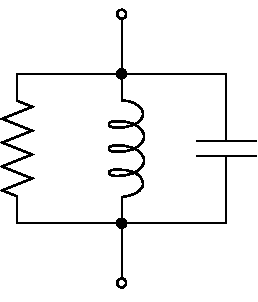
\includegraphics[]{figure1.drawio.pdf}
        \caption{LCR並列共振回路}
    \end{center}
\end{figure}

\newpage

並列共振回路に対し回路全体を流れる電流$I$\,[A]と抵抗$R$に分流する電流$I_R$\,[A]の
電流相対比$I_{ratio}$を定義する.

$$
I_{\text {ratio }} \equiv \frac{\left|I_R\right|}{|I|}
$$

$I_{ratio}$の周波数特性を同調曲線と呼ぶ.図1の並列並列共振回路においては$I_{ratio}$は

$$
I_{\text {ratio }}=\frac{1}{|Y(\omega)| R}=\frac{|Z(\omega)|}{R}=\frac{|Z(\omega)|}{\max |Z(\omega)|}
$$

ともかける.共振周波数$f_0$\,[Hz]において$I_{ratio}$は最大値1をとる.
$I_{ratio} = 1 / \sqrt[]{2}$を満たす各周波数$\omega_L$,$\omega_H$
($\omega_L < \omega_0 < \omega_H$),あるいは周波数$f_L$,$f_H$\,($f_L < f_0 < f_H$)に
対し

$$
S=\frac{\omega_0}{\omega_H-\omega_L}=\frac{f_0}{f_H-f_L}
$$

を選択度と呼ぶ.共振周波数の時のコイルまたはキャパシタに分流する電流$I$との電流比を
考えると,共振回路の$Q$は

$$
Q=\omega_0 C R=\frac{R}{\omega_0 L}=R \sqrt{\frac{C}{L}}
$$

で与えられる.このとき,

$$
Q=S
$$

が成立する.
